%!TEX program = lualatex
\documentclass[border=0mm,11pt]{standalone}
%\usepackage{color}
%\usepackage{tikz}
\usepackage[T1]{fontenc}
\usepackage[sc]{mathpazo}
\usepackage{tikz-feynman}
\tikzfeynmanset{compat=1.1.0}


\begin{document}

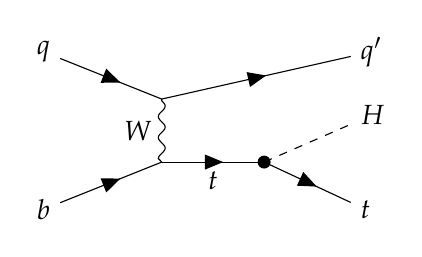
\begin{tikzpicture}[]
    \begin{feynman}
    \vertex (a) {$q$};
    \vertex [right=of a, xshift=0.0cm, yshift=-0.6cm] (b);
    \vertex [right=of b, xshift=0.9cm, yshift=0.6cm] (c) {$q'$};

    \vertex [below=of a, xshift=0.0cm, yshift=-0.5cm] (d) {$b$};
    \vertex [right=of d, xshift=0.0cm, yshift=0.6cm] (e);
    \vertex [right=of e, xshift=-0.2cm, yshift=-0.0cm] (cent);
    \vertex [right=of cent, xshift=-0.4cm, yshift=-0.6cm] (f) {$t$};

    \vertex [right=of cent, xshift=-0.4cm, yshift=0.6cm] (h) {$H$};
    \node [dot] at (cent) {};
    \diagram* {
    (a) -- [fermion] (b) -- [fermion] (c),
    (d) -- [fermion] (e) -- [fermion, edge label'=\(t\)] (cent) -- [fermion] (f),
    (b) -- [boson, edge label'=\(W\)] (e),
    (cent) -- [scalar,] (h),
    };
    \end{feynman}
\end{tikzpicture}

\end{document}